% Copyright 2007 by Till Tantau
%
% This file may be distributed and/or modified
%
% 1. under the LaTeX Project Public License and/or
% 2. under the GNU Public License.
%
% See the file doc/licenses/LICENSE for more details.


\lecture[4]{Measures of Dispersion}{lecture-text}

\subtitle{What is the scale of the data?}

\date{22 January 2015}


\begin{document}

\begin{frame}
  \maketitle
\end{frame}

% Overview: center, now spread.
% Range: not robust.
% SD: 
%   and variance: (almost) mean squared deviation
%   unaffected by shifts
%   why n-1?  ex: n=1
%   ... simulation.
% coefficent of variation
%   unaffected by changes of scale.
% visualizing
%   gaussian example
%   68%/95%/99% rule
%   earthquake example
%   note on bimodal distributions
% comparisons: robust/resistant
%   discuss



%%%%%
\begin{frame}{Overview}

    \structure{Last time:}
    measures of center.

    \vspace{3em}
    
    \structure{Today:}
    measures of dispersion. \\
    (or: ``scale'', ``spread'', \ldots)

    \vspace{3em}
    
    Already talked about one: the InterQuartile Range (IQR).

\end{frame}


%%%%%
\begin{frame}\frametitle<presentation>{Outline}
  \tableofcontents
\end{frame}


%%%%% %%%%%
\section{Measures of dispersion: the range}


%%%%%
\begin{frame}{The Range}

    The \structure{range} of a dataset is the difference between the largest and smallest observations:
    \[
        \mathrm{range}(y) = \max(y)-\min(y) .
    \]

    \vspace{3em}
    \pause

    \structure{Example:} Weight gain of lambs:
    \begin{center}
        \begin{tabular}{cccccc}
            11 & 13 & 19 & 2 & 10 & 1
        \end{tabular}
    \end{center}
    \pause
    \begin{align*}
        \mathrm{range}(y) &= 18  \\
        \mathrm{IQR}(y) &= 11
    \end{align*}

    \pause
    \vspace{2em}

    \structure{``Example:''} Weight gain of baby sharks:
    \begin{center}
        \begin{tabular}{cccccc}
            11 & 13 & 190 & 2 & 10 & 1
        \end{tabular}
    \end{center}
    \pause
    \begin{align*}
        \mathrm{range}(y) &= 189 \\
        \mathrm{IQR}(y) &= 11
    \end{align*}

    \pause
    \textbf{Observations?}

\end{frame}

\section{Standard Deviation}

%%%%%
\begin{frame}{The Standard Deviation}

    The (sample) standard deviation (\textbf{SD}) of a dataset $y$ is:
    \[
        s = \sqrt{\frac{\sum_{i=1}^n (y_i - \bar y)^2 }{ n-1 } } .
    \]


    \vspace{3em}
    \pause

    \structure{Example:} Weight gain of lambs:
    \begin{center}
        \begin{tabular}{cccccc}
            11 & 13 & 19 & 2 & \alert{8} & 1
        \end{tabular}
    \end{center}

    \pause

    \vspace{3em}

    \structure{``Example:''} Weight gain of baby sharks:
    \begin{center}
        \begin{tabular}{cccccc}
            11 & 13 & 190 & 2 & \alert{8} & 1
        \end{tabular}
    \end{center}

\end{frame}

%%%%%
\begin{frame}{The Standard Deviation}

    The (sample) standard deviation (\textbf{SD}) of a dataset $y$ is:
    \[
        s = \sqrt{\frac{\sum_{i=1}^n (y_i - \bar y)^2 }{ n-1 } } .
    \]

    \vspace{2em}
    \pause

    \structure{Unpacked}, that's:

\centering
\only<5->{Square root of ( \\} 
\only<6->{$(1-1/n)\times{}$\\} 
\only<4->{average (} 
\only<3->{sum of squared} 
\only<2->{deviations from the mean}
\only<4->{)\\} 
\only<5->{)}

\[
    \only<2>{(y_i - \bar y) }
    \only<3>{ \sum_{i=1}^n (y_i - \bar y)^2 }
    \only<4>{{\frac{\sum_{i=1}^n (y_i - \bar y)^2 }{ n } } .}
    \only<5>{\sqrt{\frac{\sum_{i=1}^n (y_i - \bar y)^2 }{ n } } .}
    \only<6->{\sqrt{\frac{\sum_{i=1}^n (y_i - \bar y)^2 }{ n-1 } } .}
\]

\end{frame}


%%%%%
\begin{frame}{Wait, $1-\frac{1}{n}$?}

The denominator is $n-1$, not $n$:
    \[
        s = \sqrt{\frac{\sum_{i=1}^n (y_i - \bar y)^2 }{ \alert{n-1} } } .
    \]

    \vspace{3em}

    Justifications:
    \begin{enumerate}
        \item Since $\bar y$ is estimated from the data, we have one less ``degree of freedom''.
        \item If $n=1$, it gives $s=\text{(undefined)}$, the right answer.
        \item It makes some math nicer (chapter 11).
        \item It works better (sometimes).
    \end{enumerate}

\end{frame}



\section{Coefficient of Variation}



%%%%%
\begin{frame}{Coefficient of variation}

    The \structure{coefficient of variation} of a dataset\\
    is the SD divided by the mean:
    \[
        \text{CV} = \frac{ s }{ \bar y } .
    \]
    \vspace{1em}

    Note: it is \emph{unitless}.

    \vspace{3em}

    \pause
    \textbf{How does CV change after rescaling the data?} \\
    Ex: change units from pounds to kilograms.

\end{frame}


\section{Visualizing}

%%%%%
\begin{frame}{Dispersion: ``width'' of the histogram}

    \begin{itemize}
        \item IQR: the middle 50\%.
        \item $\bar y \pm s$: about the middle 68\%.
        \item $\bar y \pm 2s$: about the middle 95\%.
        \item $\bar y \pm 3s$: almost everything ($>99\%$).
    \end{itemize}

    Earthquake \only<1-2>{magnitude:} \only<3>{latitude:}
    \includegraphics<1>[width=\textwidth]{quakes-hist-IQR}
    \includegraphics<2>[width=\textwidth]{quakes-hist-only}
    \includegraphics<3>[width=\textwidth]{quakes-hist-mean-sd}
    \includegraphics<4>[width=\textwidth]{quakes-lat-mean-sd}

\end{frame}


%%%%%
\begin{frame}{Comparisons}

    \begin{itemize}
        \item \textbf{range:} simple, straightforward.
        \item \textbf{IQR:} simple, robust.
        \item \textbf{SD:} not robust, uses more of the data.
    \end{itemize}

    \vspace{2em}
    \pause

    \begin{quote}
        \ldots the SD is the basis for most standard classical statistical methods. The SD enjoys its status for various technical reasons\ldots The developments in later chapters will emphasize classical statistical methods [\ldots so] we will rely primarily on the mean and SD rather than other descriptive measures.
    \end{quote}

    \vspace{3em}
    \pause

    If different methods give you \emph{different answers},
    you should think about \emph{why},
    and which is more appropriate.

\end{frame}

%%%%%
\begin{frame}{Linear transformations}

    Suppose our data $y$ are in $^{\circ}$C, and we change them to $z$, in $^{\circ}$F:
    \[
        z_i = 32 + 1.8 y_i
    \]

    \vspace{2em}

    How does this change the mean and SD?
    (think in terms of \emph{shape of the histogram})

    \pause

    \begin{align*} 
        \bar z &= 32 + 1.8 \bar y  \\
        s_z &= 1.8 s_y
    \end{align*} 

\end{frame}


%%%%%
\begin{frame}{Nonlinear transformations:}

    \begin{itemize}
        \item $\bar y \pm s$: about the middle 68\%.
        \item $\bar y \pm 2s$: about the middle 95\%.
        \item $\bar y \pm 3s$: almost everything ($>99\%$).
    \end{itemize}

    Distribution of $\sqrt{\text{magnitude}}$:

    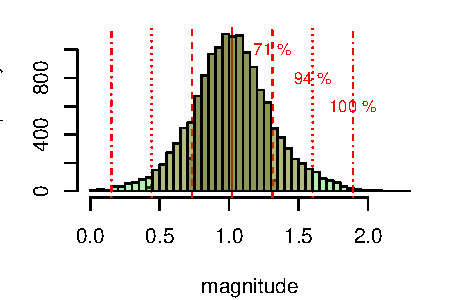
\includegraphics[width=\textwidth]{quakes-sqrt-hist-mean-sd}

\end{frame}



% Overview: center, now spread.
% Range: not robust.
% SD: 
%   and variance: (almost) mean squared deviation
%   unaffected by shifts
%   why n-1?  ex: n=1
%   ... simulation.
% coefficent of variation
%   unaffected by changes of scale.
% visualizing
%   gaussian example
%   68%/95%/99% rule
%   earthquake example
%   note on bimodal distributions
% comparisons: robust/resistant
%   discuss

\section<article>{Summary}
\section<presentation>*{Summary}

\begin{frame}{Summary}
  \begin{enumerate}
    \item The range summarizes how widely the data are spread,
    \item but the IQR better summarizes the typical spread.
    \item The SD is \emph{almost} the root mean square deviation,
    \item and is a less robust, but sometimes better, measure of dispersion.
    \item It is useful to think about these as concrete aspects of the histogram.
    \item The SD and CV do not change under multiplicative rescaling,
    \item and the mean and SD don't change under additive shifts.
  \end{enumerate}
\end{frame}

% homework
\begin{frame}{Homework}
  \begin{center}

    2.6.2

  \vspace{2em}

    2.6.3

  \vspace{2em}

    2.7.1
  
  \end{center}
\end{frame}


\end{document}
